\chapter{Software implementation}\label{cap.software}

In this chapter, we explain the algorithm that we have designed for solving the visual people tracking problem and its software implementation. 

\section{System overview}

The main contribution of this work is to develope a tracking algorithm that utilizes neural network and do not miss the real time objective. To do so it combines people detection using a neural network, somehow, slow but very accurate, and feature tracking, very quick but prone to drift. 

The architecture of the system is summarized in the diagram \ref{software1}, it has a sequence of frames as input and a CSV file as output. This file has the structure of the MOT's evaluation software requires. We divided the computing in two threads, the object detector thread and the main thread. The first is responsible of given a frame compute their pedestrian detections and send them to the tracking thread, and the second one, given a detection it computes the tracking procedure, in adition, when a new detection appears it combines with the tracker, this is called data association, and finally it saves the results of the algorithm.



\begin{figure}[H]
\centering         
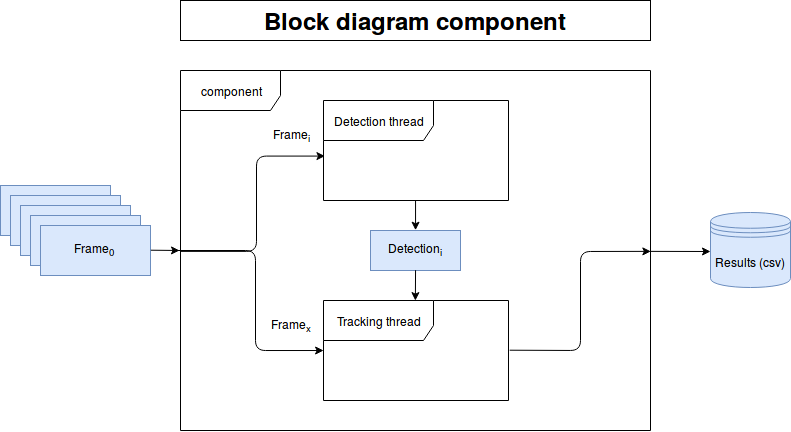
\includegraphics[width=8cm]{flows/bloque.png}
\caption{Block diagram of the component.} \label{software1}
\end{figure}


Temporally the system works as follows, when the algorithm starts, first of all it launches the object detector thread, it begins to compute the detections of the first frame. Meanwhile, the tracking thread is idle, waiting for the detections. When the object detector finishes, it sends the detection to the tracking thread and at the same time starts to compute the detections of a predefined next frame. When the tracking thread has got a detection, it begins to compute the tracking between frames. Considering that the thread are not syncronized, the object detection thread goes ahead of the tracking thread it will have a detection when the tracking thread could not incorporate, thus, saves the detections and starts to compute the next one. When the tracking thread arrives to a frame that has a detection it has a mechanism to mix detection with trackets, what is called data association module, after running this module it will continue comuting the tracking. We can observe this temporal process in the next figure \ref{software2}, when $T$ represents a temporal step. When the object detector thread finishes computing all the detections it will \textit{die}. The tracking thread computes their task previously stated till it does not have any frame to process.


\begin{figure}[H]
\centering         
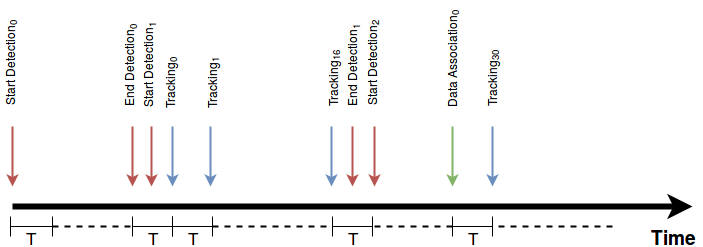
\includegraphics[width=14cm]{timesDiagram/timing.png}
\caption{Timing of the component.} \label{intro1}
\end{figure}


In the figure \ref{introTracking3} there is a flow chart of the algorithm and it summarzizes as follows: The object detector thread reads images, processes the forward pass of the neural network and saves the detections in the shared buffer, it repeats this sequence until it has processed all the predefined list of images. In another hand, the main tread, activates the object detector thread and waits till it gets the first detection, after this, it starts the tracking algorithm. It reads the images and computes the motion of all the regions of interest. However, at beginning of each cycle it checks whether it has newer detection to mix in. This is the main operating mode of the algorithm and it summarizes in the figure \ref{system1}. In the next sections we will develope in detail these parts. 

\begin{figure}[H]
	
\centering

\subfigure[Main thread.]{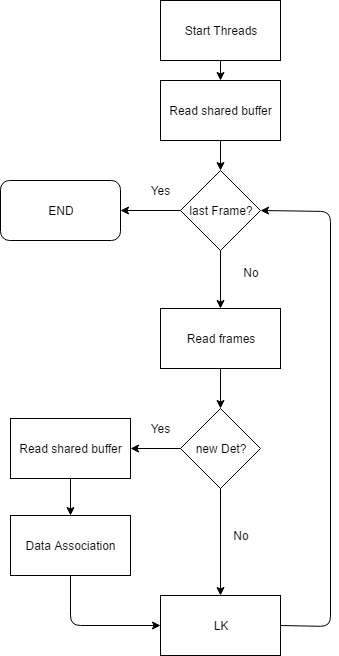
\includegraphics[width=5cm]{flows/arc.png}}
\subfigure[Object detector thread.]{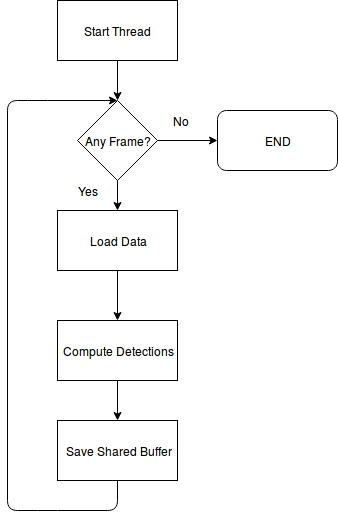
\includegraphics[width=5cm]{flows/detetc.png}}\\


\caption{Flow chart of the system.}
\label{introTracking3}
\end{figure}

We represent each person with a bounding box, in this bounding box we extract some features and compute how they move through the frames, based on the movement of those features we will infer the movement of the bounding box, therefore, the movement of the person.

\section{System design}

In this section we explain the parts of the algorithm in detail.

\subsection{Object detecion by neural networks}



As we stated previously we compute the pedestrian detector based on a CNN. This types of systems are very accurate but slow. We are constraint by its execution time, it takes $0.92$ seconds for compute a detection, this allows us to get a new detection after $30$ frames. Thus,  the object detection computes a list of frame's index to compute the detection.



\begin{algorithm}
\caption{Object detection thread}\label{euclid}
\begin{algorithmic}[1]
\Procedure{Detection}{}
%\State $A tracker prodcues a trajectory by tracking the point forward in time$
%\State $network \gets \textit{patlen}$
\State $network = network.init()$
\State $FPS = 30$
\State $FRAMES SEQUENCES = num of files(sequences)$
\State $LIST_INDEXs = createList(FPS,FRAMES_SEQUENCES)$
\For {(each object $LIST_INDEX$)}
\State $image = read()$
\State $detection = network.forward(image)$
\State $sharedVariable = detection$
\EndFor
\EndProcedure
\end{algorithmic}
\end{algorithm}

We selected the Single shot multibox detector as object detector, in section we explain why chose this detector. Finally, in \ref{objectDetector1} we can observe the result of this step.


\begin{figure}[H]
\centering         
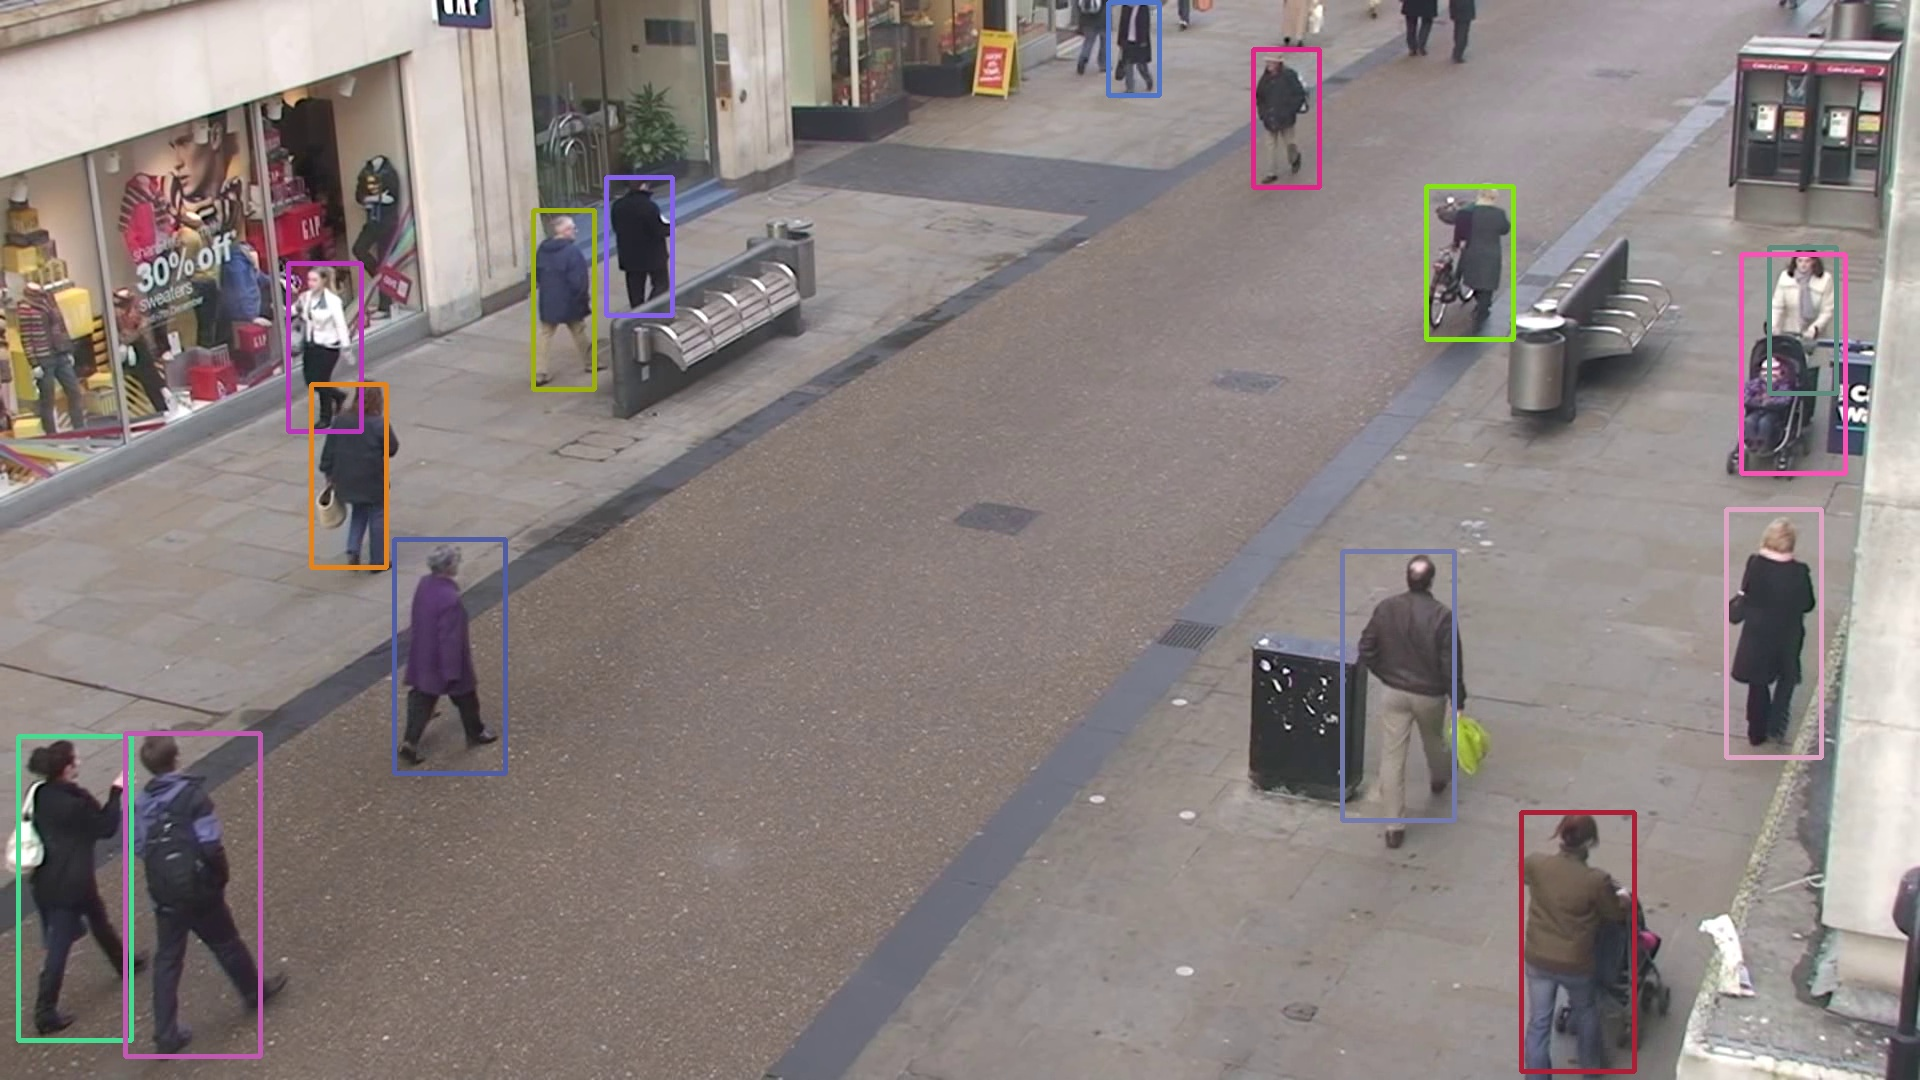
\includegraphics[width=10cm]{intro/deteccions.jpg}
\caption{Detections of the algorithm.} \label{objectDetector1}
\end{figure}


\subsection{Feature tracking}


The tracking module is inspired by the well-known tracking algorithm \textit{MedianFlow} by Zalal et al\cite{medianFlow} with his correspondent implementation in Python\cite{medianFlowPython}. Next we explain the tracking module in details.



The essence of the tracking thread it is the tracking module, called LK in the figure \ref{introTracking3}. It stands for Lucas-Kanade algorithm, due it is the method that we used in this work. This module for each detection computes its displacement by computing the displacement of the features inside this bounding box.





\begin{algorithm}
\caption{Object detection thread}\label{euclid}
\begin{algorithmic}[1]
\Procedure{Detection}{}
%\State $A tracker prodcues a trajectory by tracking the point forward in time$
%\State $network \gets \textit{patlen}$
\State $network = network.init()$
\State $FPS = 30$
\State $FRAMES SEQUENCES = num of files(sequences)$
\State $LIST_INDEXs = createList(FPS,FRAMES_SEQUENCES)$
\For {(each object $LIST_INDEX$)}
\State $image = read()$
\State $detection = network.forward(image)$
\State $sharedVariable = detection$
\EndFor
\EndProcedure
\end{algorithmic}
\end{algorithm}



For extracting the features, we use the OpenCV routine \texttt{goodFeaturesToTrack()}, this function determines strong corners on an image, according the Shi Tomasi method. His parameters are the following:
 
\begin{itemize}

\item \texttt{image}, input image

\item \texttt{maxCorners}, maximum number of corners to return. If there are more corners than are found, the strongest of them is returned.
\item \texttt{qualityLevel}, parameter characterizing the minimal accepted quality of image corners.
\item \texttt{minDistance}, minimum possible Euclidean distance between the returned corners.
\item \texttt{mask}, optional region of interest.
\item \texttt{blockSize}, Size of an average block for computing a derivative covariation matrix over each pixel neighborhood.
\item \texttt{useHarrisDetector},  Parameter indicating whether to use a Harris detector.
\item \texttt{k},  Free parameter of the Harris detector.

\end{itemize}


\begin{figure}[H]
\centering         
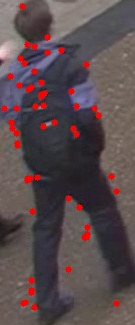
\includegraphics[width=3cm]{implementation/pointsEQU.jpg}
\caption{Detections of the algorithm.} \label{objectDetector1}
\end{figure}


\begin{figure}[H]
\centering         
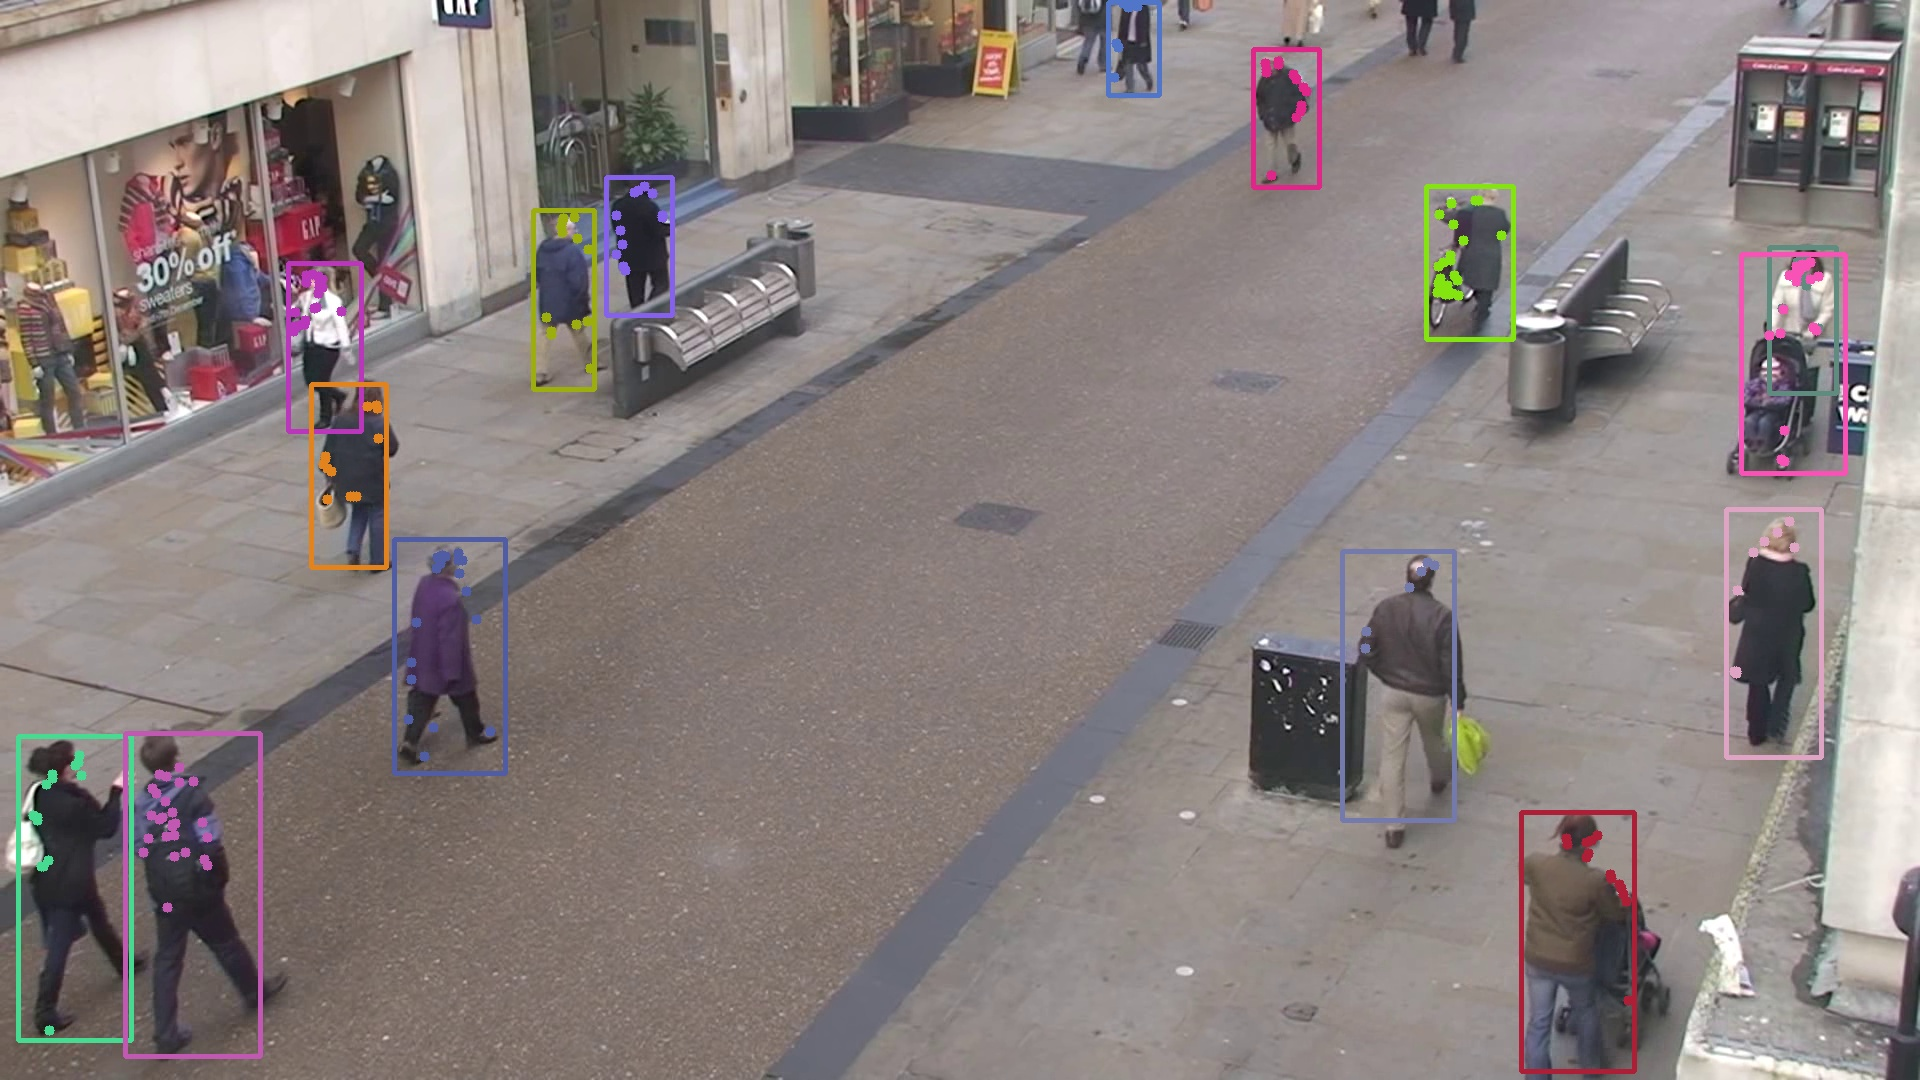
\includegraphics[width=10cm]{intro/pounts.jpg}
\caption{Detections of the algorithm.} \label{objectDetector1}
\end{figure}

 
%\begin{algorithm}
%\caption{Forward-backward method}\label{euclid}
%\begin{algorithmic}[1]
%\Procedure{FB}{}
%\State $A tracker prodcues a trajectory by tracking the point forward in time$
%\State $i \gets \textit{patlen}$
%%\BState \emph{top}:
%\If {$i > \textit{stringlen}$} \Return false
%\EndIf
%\State $j \gets \textit{patlen}$
%%\BState \emph{loop}:
%\If {$\textit{string}(i) = \textit{path}(j)$}
%\State $j \gets j-1$.
%\State $i \gets i-1$.
%\State \textbf{goto} \emph{loop}.
%\State \textbf{close};
%\EndIf
%\State $i \gets i+\max(\textit{delta}_1(\textit{string}(i)),\textit{delta}_2(j))$.
%\State \textbf{goto} \emph{top}.
%\EndProcedure
%\end{algorithmic}
%\end{algorithm}




Motion


To compute the flow, we used the OpenCV's routine \texttt{calcOpticalFlowPyrLK()}, this function implements a sparse iterative version of the Lucas-Kanade optical flow with pyramids. And his parameters are the following:
 
\begin{itemize}

\item \texttt{prevImg}, first image.
\item \texttt{nextImg}, second image.
\item \texttt{prevPts}, vector of 2D points for which the flow needs to be found. 
\item \texttt{nextPts}, output vector of 2D points containing the calculated new positions of input features in the second image. 
\item \texttt{status}, output status vector, it tells you whether the flow has been found.  
\item \texttt{err}, each element of the vector is set to an error for the corresponding feature.
\item \texttt{winSize}, size of the search window at each pyramid level. 
\item \texttt{maxLevel}, number of pyramid levels.  
\item \texttt{criteria}, parameter, speifying the termination criteria of the iterative search algorithm.
\end{itemize}



In the next figure we can observe the matching of the features in subsequents frames.

\begin{figure}[hptb]
\centering         
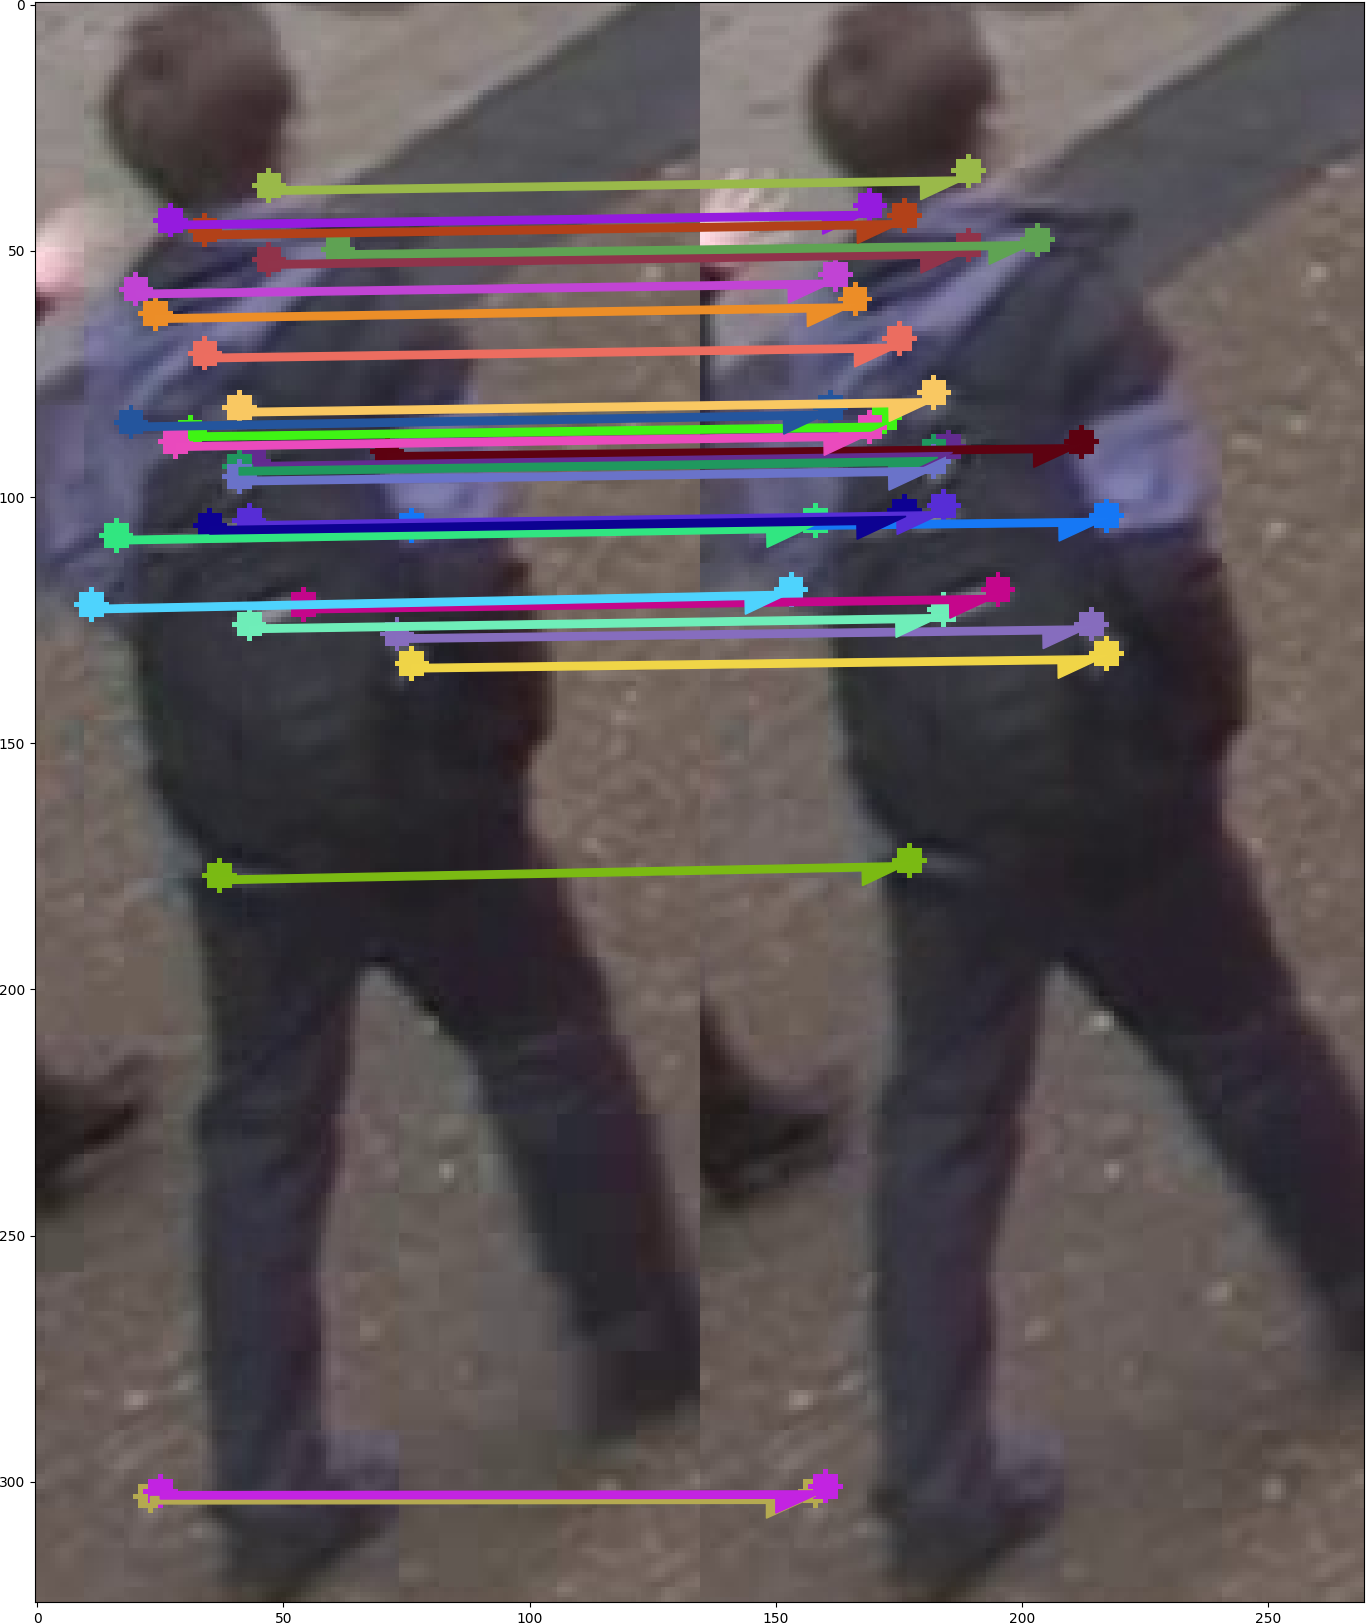
\includegraphics[width=0.3\linewidth]{implementation/matching.png}
\caption{Image and motion vectors.} \label{motion1}
\end{figure}




\begin{figure}[H]
\centering         
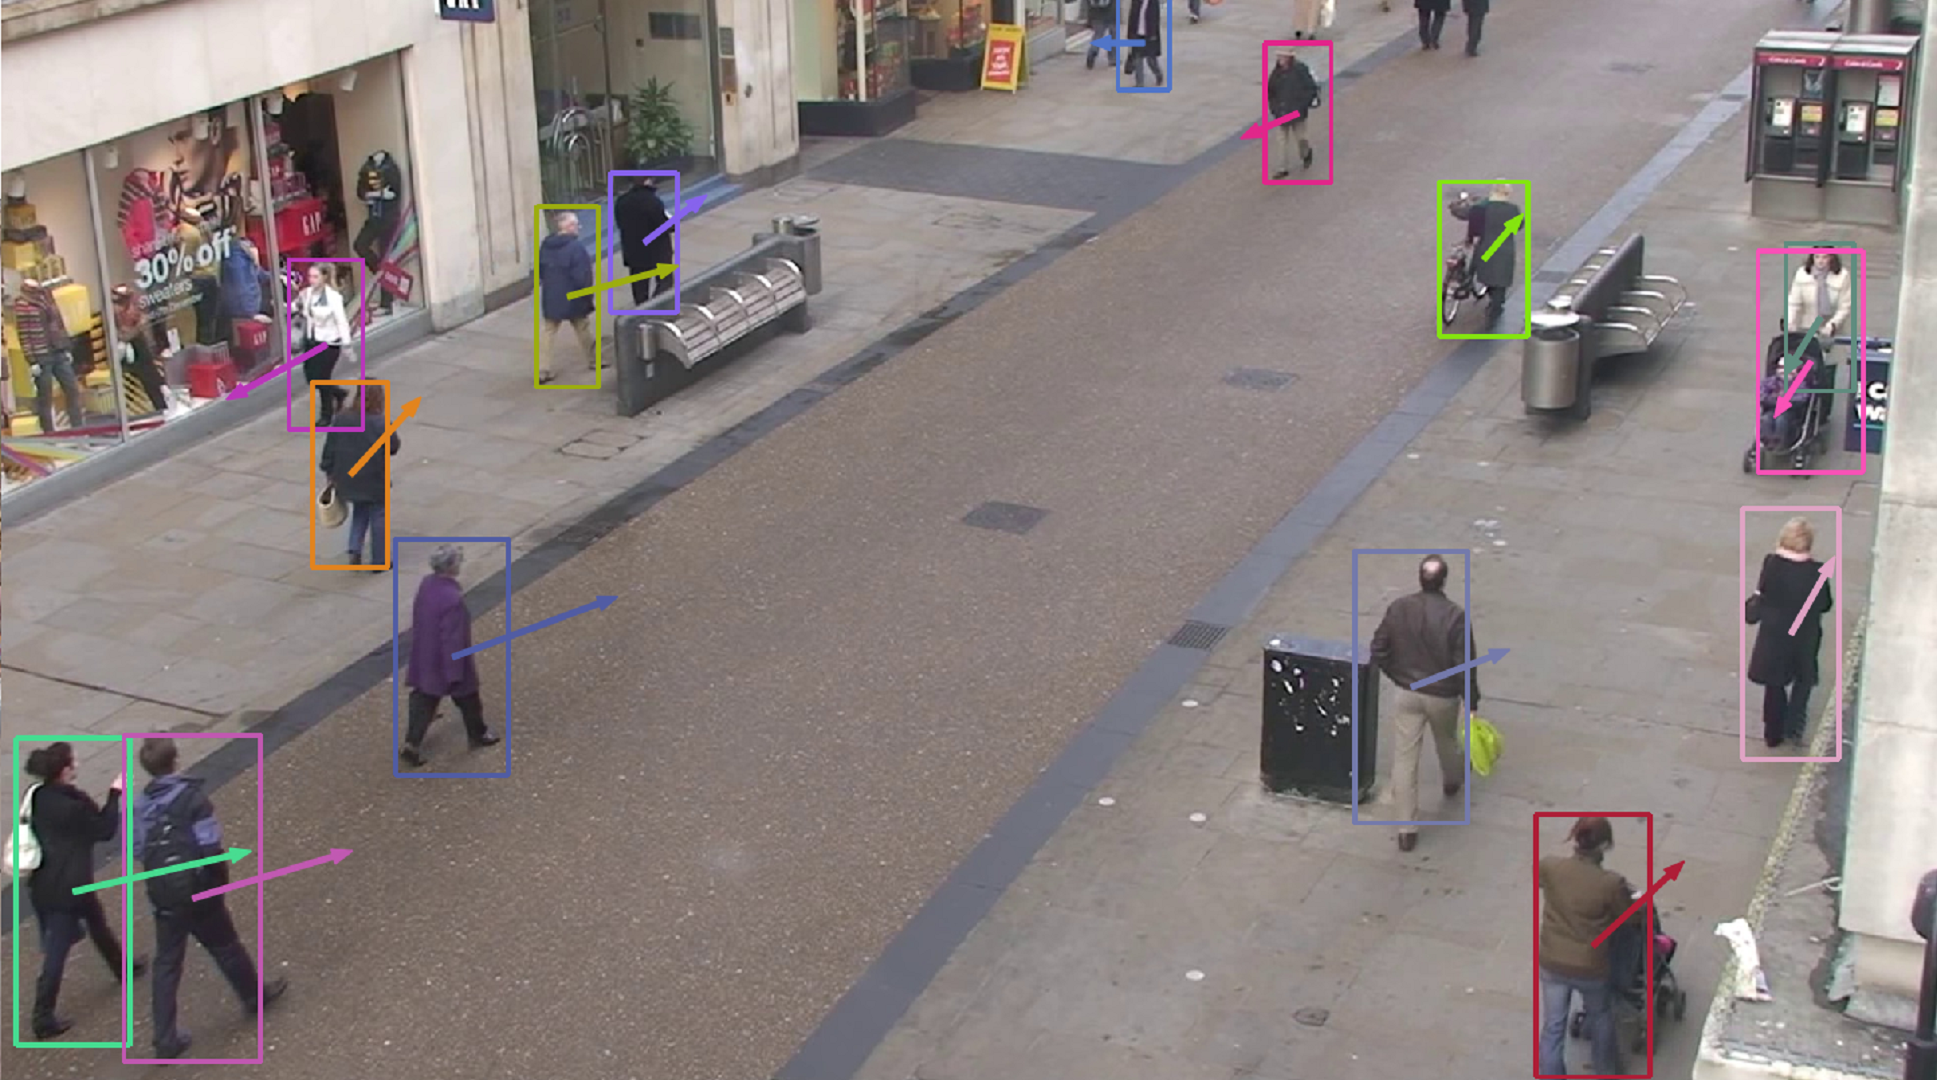
\includegraphics[width=10cm]{intro/alcover2.png}
\caption{Detections of the algorithm.} \label{objectDetector1}
\end{figure}



Problemas

Next we erased this points, we compute the motion as the median of all the contibutions displacement vectors in each dimension. Also, the scale change is computed as follows: for each pair of points, a ratio between current point distance and previous point distance is computed, bounding box scale change is defined as the median over these ratios. 

At this point, we have an implementation of the tracking algorithm given a set of bounding boxes. Nevertheless, we notice running our algorithm on the dataset, that the bounding box could compute the motion of the assigned pedestrian including the points belonging to another pedestrian who appears also in the bounding box. This interaction will cause a wrong estimation of the movement of the target and eventually the pedestrian will not be embedded by the bounding box. We can observe this event in figure \ref{traccs}.


\begin{figure}[H]
\centering         
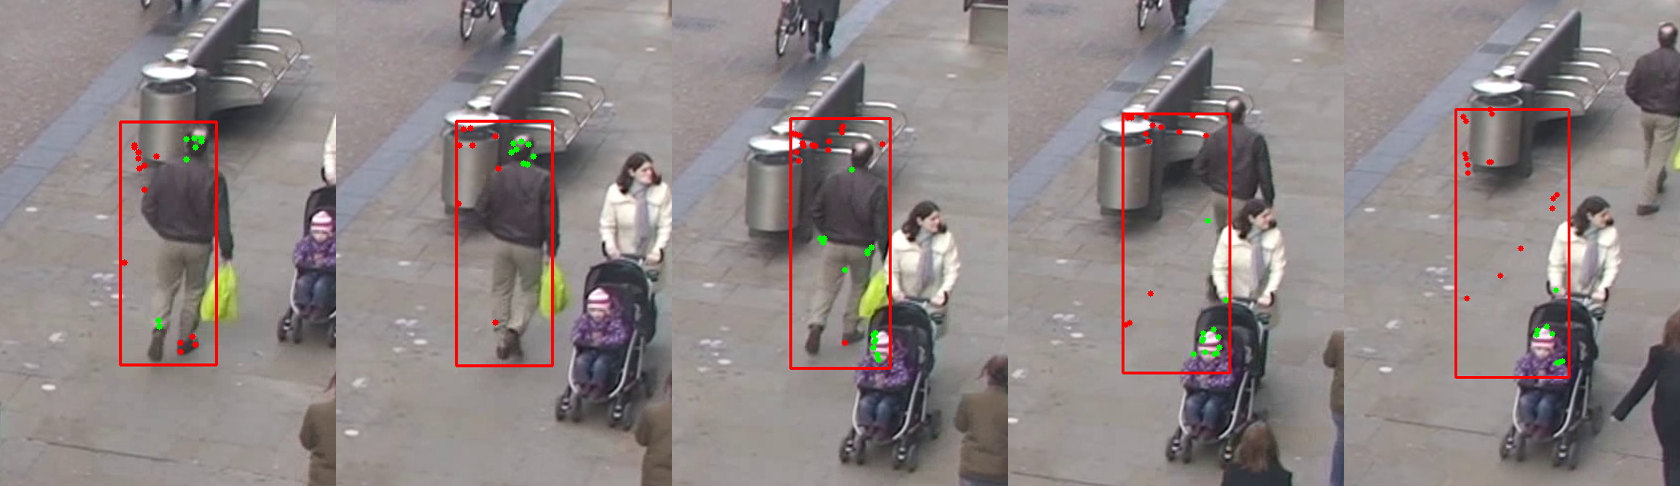
\includegraphics[width=0.9\linewidth]{velocidadas/mateuPont.png}
\caption{Tracking failure.} \label{traccs}
\end{figure}


So, we need a mechanism to detect these failures, therefore we studied how the motion algorithm behaves in these situations. When it has got a trajectory without crossing with other pedestrian, the vertical and horizontal displacement behave like a damping sine wave (if it goes away of the camera)  or amplified sine wave ( if it goes closer to the camera ). But when it has got an interference with another pedestrian, it has an steep change in that wave. We can measure that change as the differences between the current displacement and the previous one normalized by current displacement, if this value overtake a thresolhd, we consider that tracket as a lost tracket. We can observe this process in the next figure \ref{traccs23}, it belongs to previous trajectory \ref{traccs} 


\begin{figure}[H]
\centering         
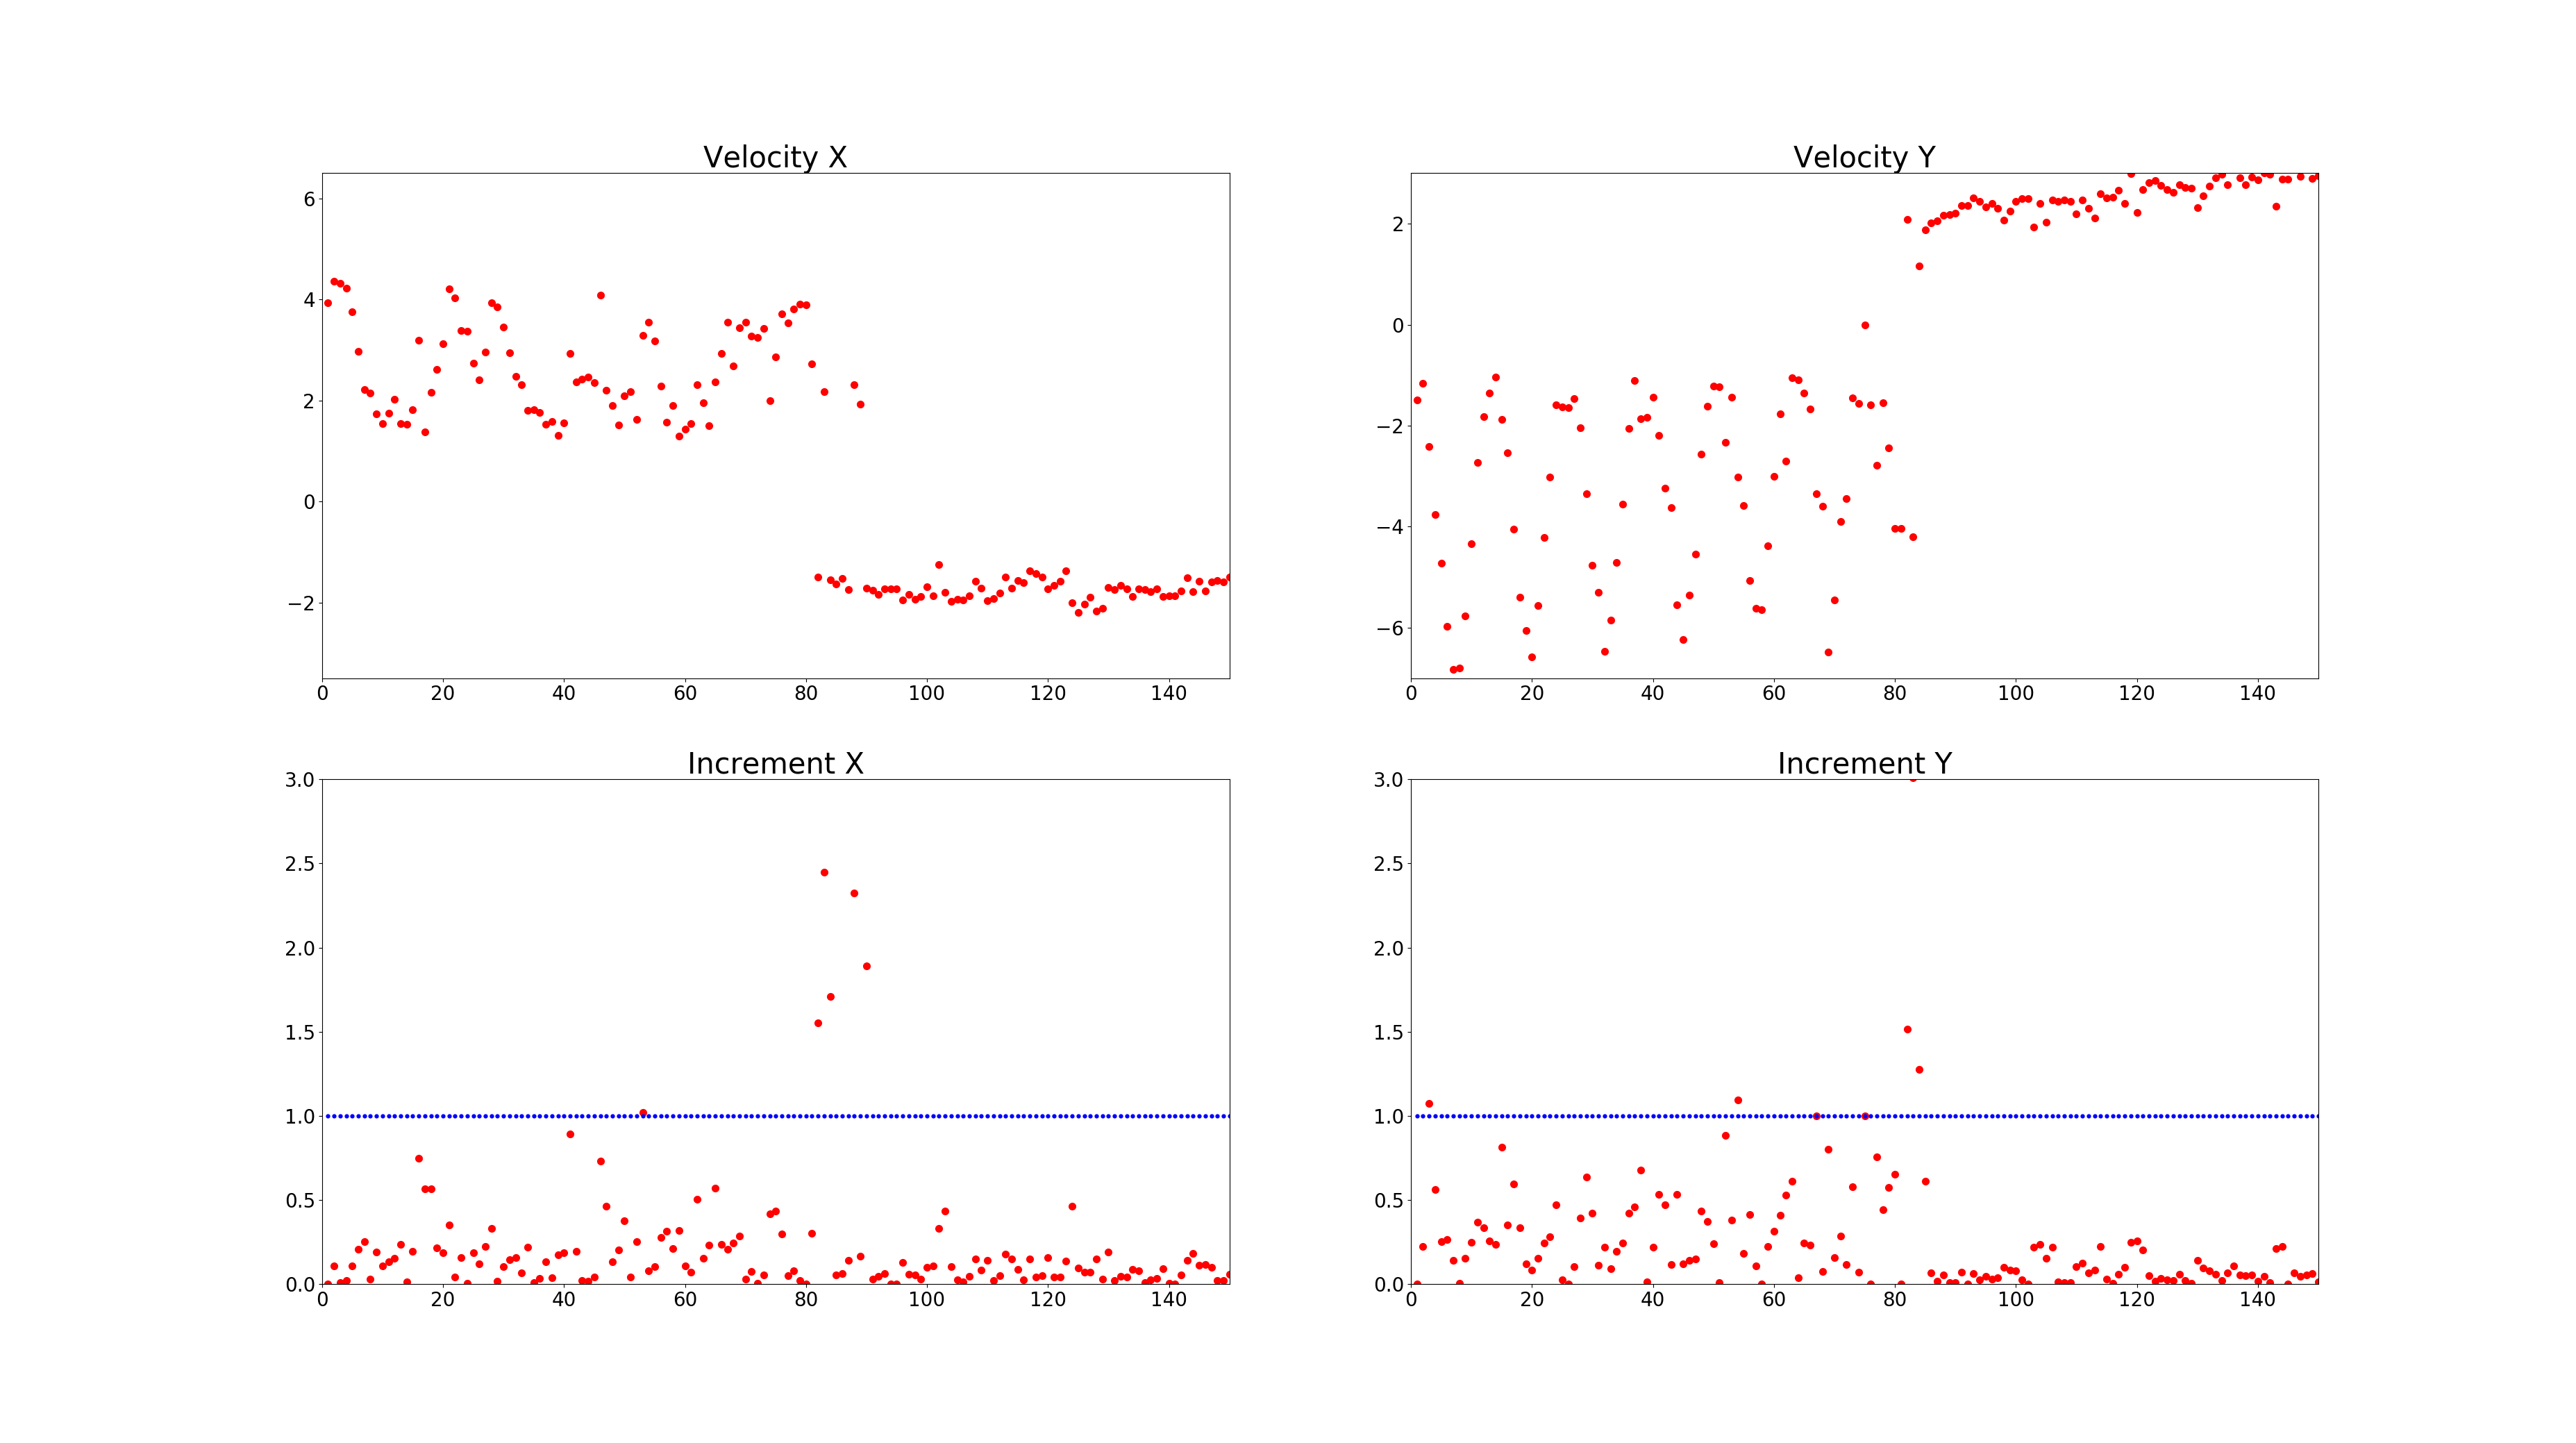
\includegraphics[width=0.9\linewidth]{velocidadas/bad_threshold.png}
\caption{Tracking failure.} \label{traccs23}
\end{figure}


In contrast, when it does not cross with another pedestrian, the displacement does not get disrupt, then the normalized different with the previous displacement gets a low value, we can observe this process in figure \ref{motion2nocoorrect}. We set a threshold to notice this interference and delete this bounding box. We delete them from the current tracking execution, but we save the bounding box for following processings.

\begin{figure}[H]
		
\centering

\subfigure[Trajectory.]{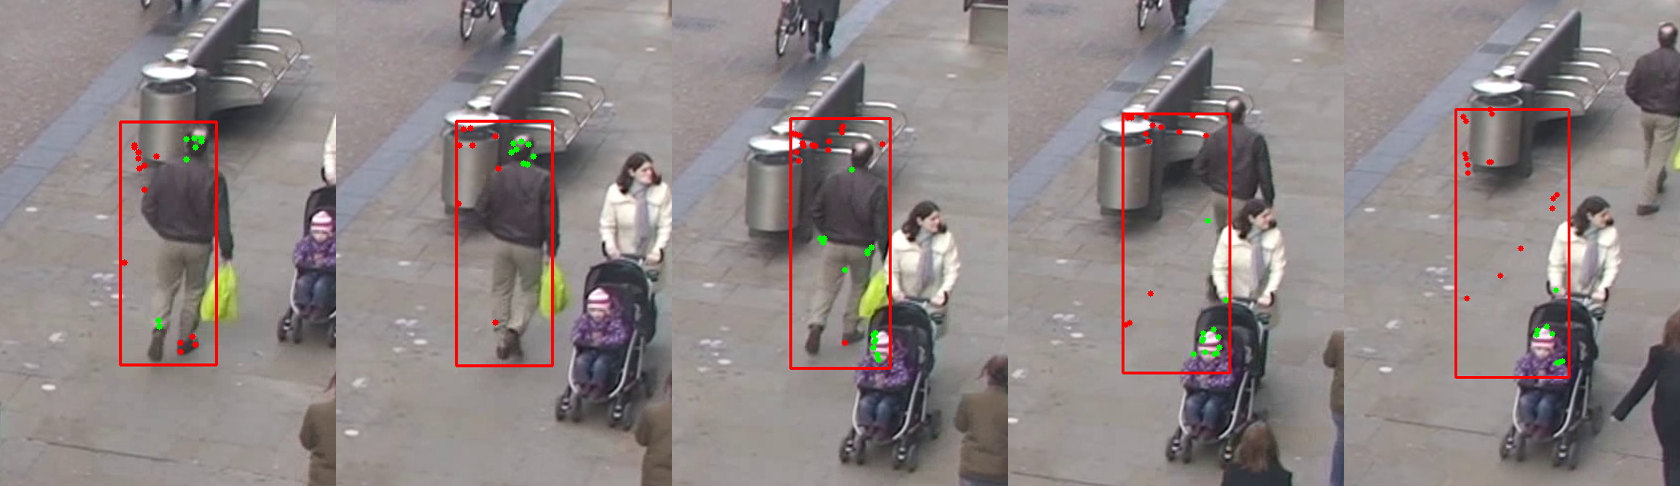
\includegraphics[width=15cm]{velocidadas/mateuPont.png}}\\
\subfigure[Plots movement.]{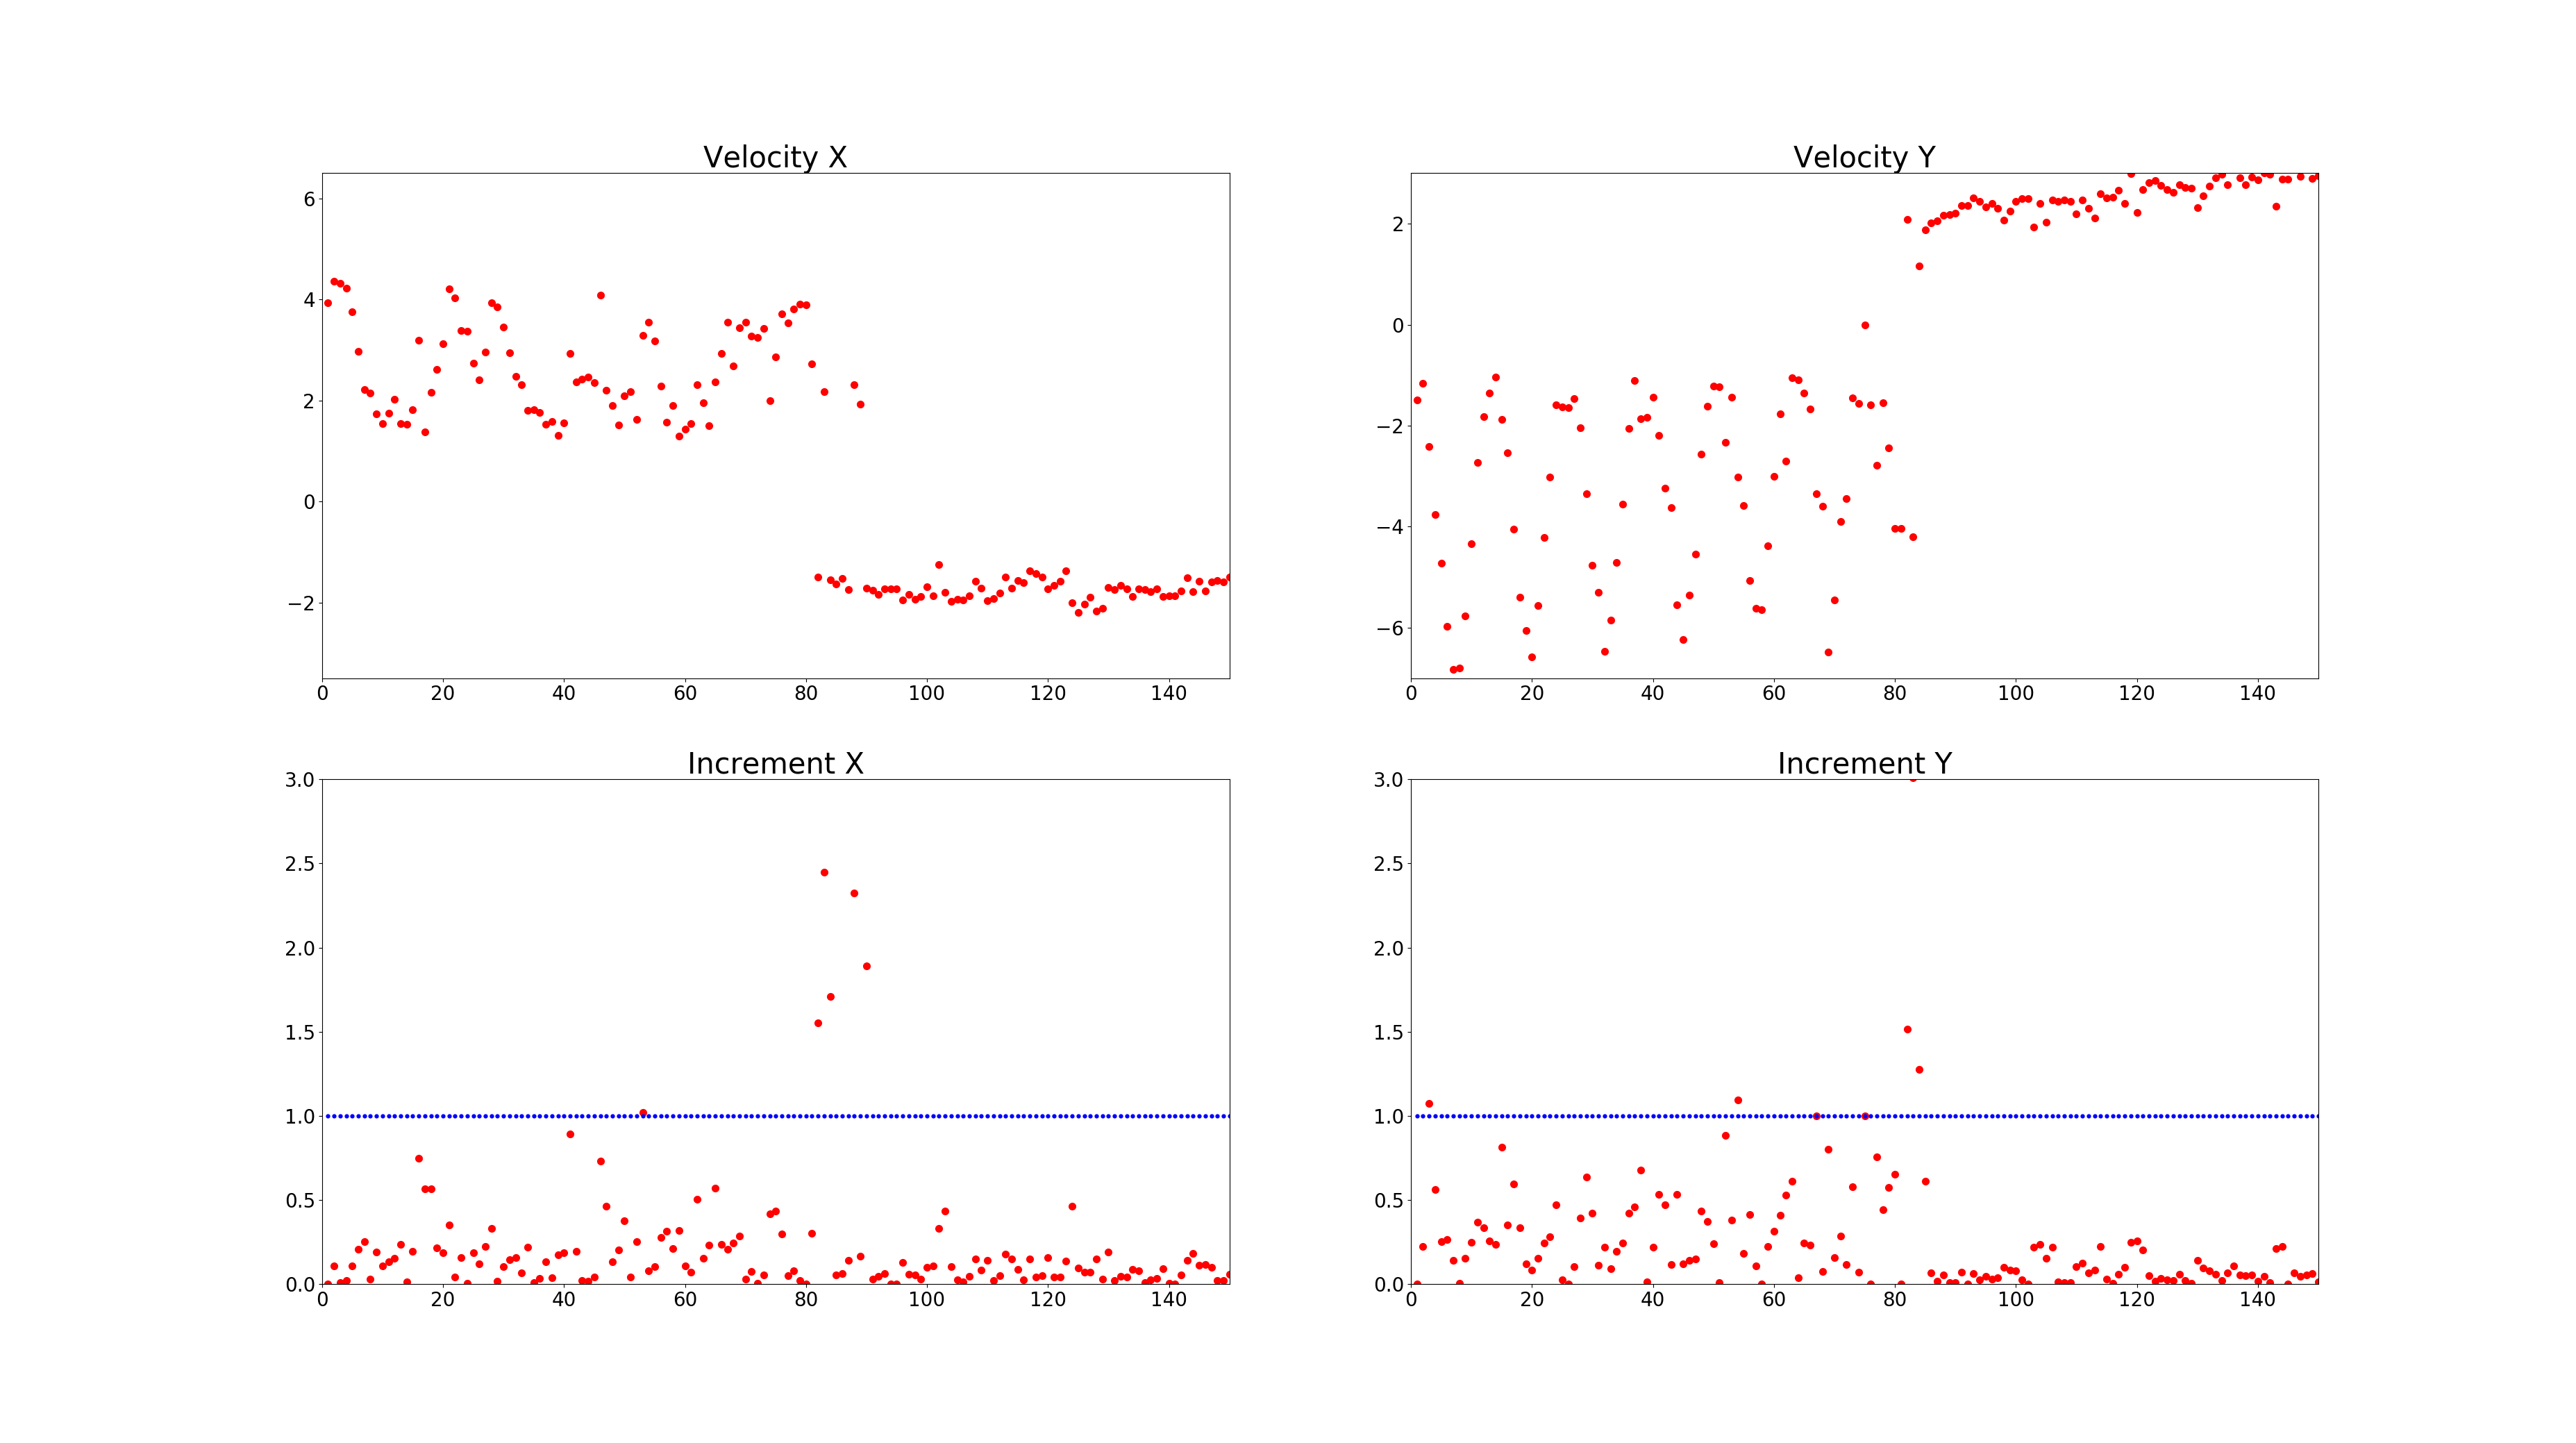
\includegraphics[width=16cm]{velocidadas/bad_threshold.png}}\\
\caption{Wrong trajectory.}
\label{motion2nocoorrect}
\end{figure}













\subsection{Data association}

Once we computed the trajectories, in the next iteration we might have to add a detection, so we need a module to combine these trajectories with detections. Thus, for each pedestrian we distinguish three situations:

\begin{itemize}



\item \textbf{Situation 1}, the tracket has got a nearby detection, then the detection replace the tracket bounding box. This is what is called spatio-temporal constraint.

\item \textbf{Situation 2}, the tracket has not got a nearby detection, then the bounding box tracket continues.

\item \textbf{Situation 3}, the pedestrian has not got a tracket but has got a detection. In this case we need to decided whether this pedestrian is new in the scene or it has been seen before ( it is a lost tracket ).

\end{itemize}

We can observe the procedure for situations number one and two in the figure \ref{data1}, in green colour we can observe the detections and in blue colour the trackets. We defined nearby as the distance between the centres of the boundings boxes, this distance has to be lower than a threshold to be consider nearby. 

\begin{figure}[hptb]
\centering         
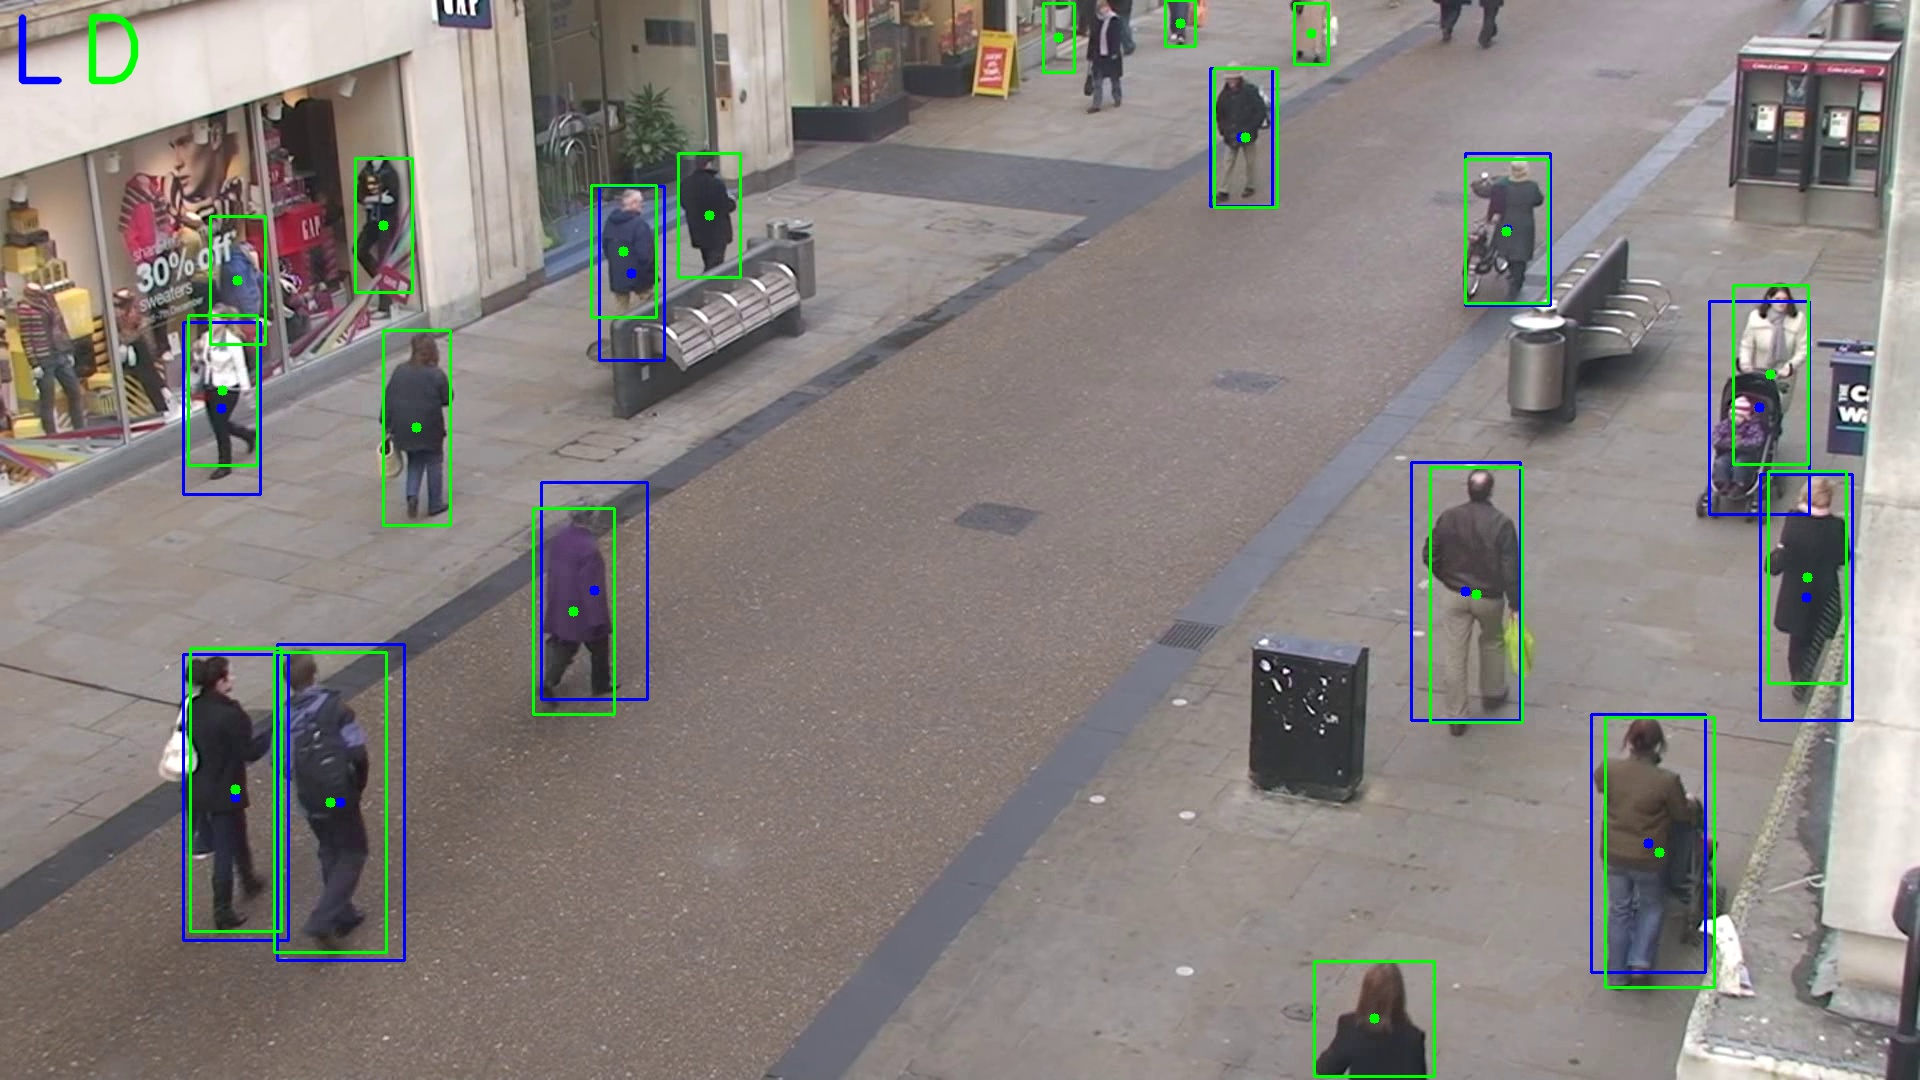
\includegraphics[width=12cm]{lucasKanade/dataAssociation.jpg}
\caption{Spatio-temporal data association.} \label{data1}
\end{figure}


\begin{figure}[hptb]
\centering         
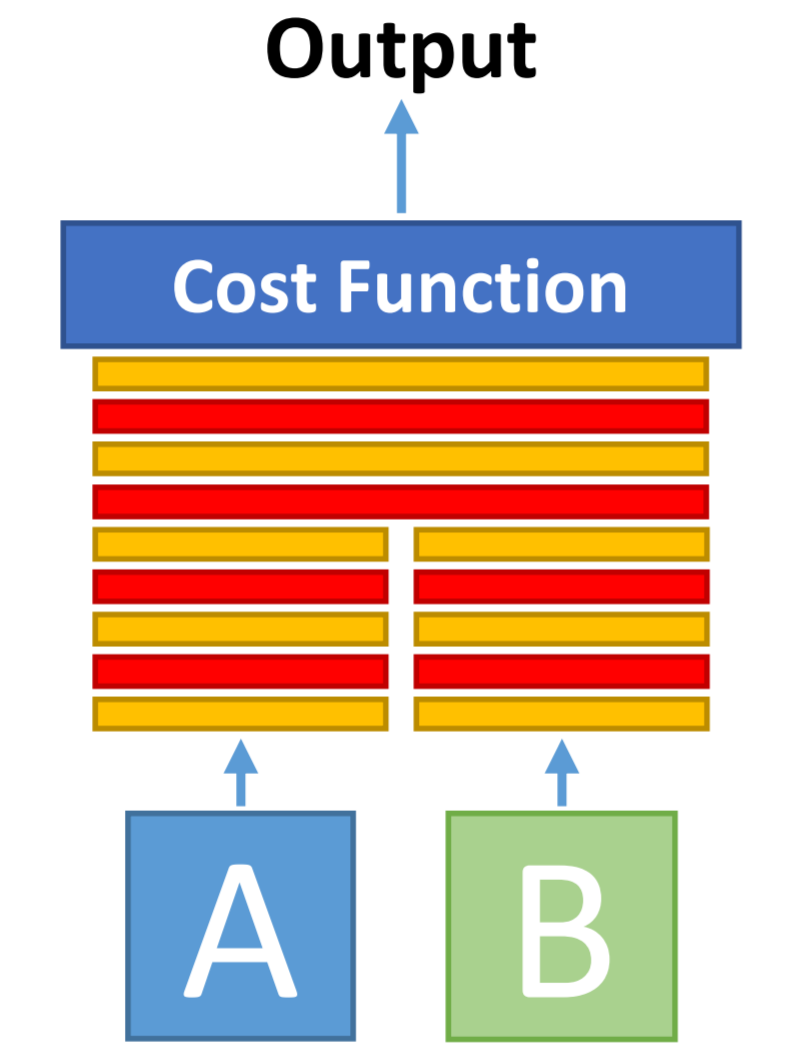
\includegraphics[width=3cm]{siamese/retall2.png}
\caption{Spatio-temporal data association.} \label{data1}
\end{figure}




